\chapter{Realisierung des Systems} \todo{ab hier alle weiteren noch Abkürzungscheck}
Zu Beginn der Realisierung erfolgt die Anordnung aller benötigten Buchstaben für die verschiedenen Funktionen und Wortdarstellungen. 
Ziel ist die Umsetzung eines möglichst kompakten und quadratischen Rasters.
Die erste Konzeptentwicklung erfolgt auf einem Tablet. 
Dabei werden die Positionen der einzelnen Buchstaben sowie deren Zuordnung zu den jeweiligen Funktionen skizziert. 
Diese Vorgehensweise ermöglicht eine flexible Anpassung des Layouts, da die Buchstaben und Symbole noch verschoben und umpositioniert werden können.
Das Ergebnis der Konzeptentwicklung ist in Abbildung~\ref{fig:Konzeptentwicklung} dargestellt.
\begin{figure}[H]
	\centering
	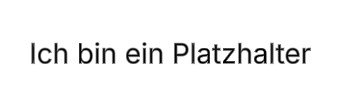
\includegraphics[width=0.3\linewidth]{inhalt/bilder/Platzhalter.jpg}
	\caption{Dargestelt ist der Schaltplan der Wortuhr mit allen angeschlossenen Komponenten und Pinbelegung des ESP32-C6.}
	\label{fig:Konzeptentwicklung}
\end{figure}

Zur Bestimmung der minimal nötigen Buchstabengröße wird ein empirischer Ansatz gewählt. 
Hierfür werden Testdrucke mit unterschiedlichen Schriftgrößen erstellt.
Das entscheidende Kriterium ist die gute Lesbarkeit aus einer Entfernung von etwa 5 m. 

Auf Basis der ermittelten Schriftgröße geht zum einen die Gesamtgröße der Wortuhr hervor.
Weiterhin kann damit der Abstand ermittelt und leicht angepasst werden, den die \gls{led}s voneinander haben müssen, damit eine \gls{led} je Buchstabe platziert wird.
Damit kann das passende \gls{led}-Band gewählt werden auf welchem die \gls{ws2812b}-\gls{led}s integriert sind.
So muss nicht jede \gls{led} einzeln verlötet werden.  
Zuletz bildet dies die Grundlage für die Aufteilung der Bauteile im Hinblick auf den Fertigungsprozess. 
Da das verfügbare Druckbett des verfügbaren \gls{3ddrucker} auf ein Volumen von 250 mm × 250 mm × 250 mm begrenzt ist, erfolgt eine entsprechende Segmentierung der Konstruktion und die Frontplattenbauteil können konstruiert werden.